\documentclass[notheorems,mathserif,table,compress]{beamer}  %dvipdfm选项是关键,否则编译统统通不过
%%------------------------常用宏包------------------------
%%注意, beamer 会默认使用下列宏包: amsthm, graphicx, hyperref, color, xcolor, 等等
\usepackage{fontspec,xunicode,xltxtra}  % for XeTeX
\usepackage{graphicx}
\usepackage{fancybox}
\usepackage{comment}
\usepackage{booktabs}
\usepackage{colortbl}
\usepackage{tcolorbox}
\usepackage{pifont}
\usepackage{multirow}
\usepackage{multicol}
%%------------------------ThemeColorFont------------------------
%% Presentation Themes
% \usetheme[<options>]{<name list>}
\usetheme{Madrid}
%% Inner Themes
% \useinnertheme[<options>]{<name>}
%% Outer Themes
% \useoutertheme[<options>]{<name>}
\useoutertheme{miniframes} 
%% Color Themes 
% \usecolortheme[<options>]{<name list>}
%% Font Themes
% \usefonttheme[<options>]{<name>}
\setbeamertemplate{background canvas}[vertical shading][bottom=white,top=structure.fg!7] %%背景色, 上25%的蓝, 过渡到下白.
\setbeamertemplate{theorems}[numbered]
\setbeamertemplate{navigation symbols}{}   %% 去掉页面下方默认的导航条.

\usepackage{zhfontcfg}
\usepackage{subfigure}
\usepackage{pgf}
\usepackage{color}
\usepackage{caption}

%\setsansfont[Mapping=tex-text]{文泉驿正黑}  %% 需要fontspec宏包
     %如果装了Adobe Acrobat,可在font.conf中配置Adobe字体的路径以使用其中文字体
     %也可直接使用系统中的中文字体如SimSun,SimHei,微软雅黑 等
     %原来beamer用的字体是sans family;注意Mapping的大小写,不能写错
     %设置字体时也可以直接用字体名,以下三种方式等同:
     %\setromanfont[BoldFont={黑体}]{宋体}
     %\setromanfont[BoldFont={SimHei}]{SimSun}
     %\setromanfont[BoldFont={"[simhei.ttf]"}]{"[simsun.ttc]"}
%%------------------------MISC------------------------
\graphicspath{{figures/}}         %% 图片路径. 本文的图片都放在这个文件夹里了.
%%------------------------正文------------------------
%\pgfputat{\pgfxy(3,-6)}{\pgfbox[centering,base]{\includegraphics[width=2cm,height=2cm]{figures/ouc}}}
\begin{document}

\XeTeXlinebreaklocale "zh"         % 表示用中文的断行
\XeTeXlinebreakskip = 0pt plus 1pt % 多一点调整的空间
%%----------------------------------------------------------
%% This is only inserted into the PDF information catalog. Can be left
%% out.
%%%
%% Delete this, if you do not want the table of contents to pop up at
%% the beginning of each subsection:

\AtBeginSection[]{                              % 在每个Section前都会加入的Frame
  \frame<handout:0>{
    \frametitle{下一节内容}\small
    \tableofcontents[current,currentsubsection]
  }
}
\AtBeginSubsection[]                            % 在每个子段落之前
{
  \frame<handout:0>                             % handout:0 表示只在手稿中出现
  {
    \frametitle{下一节内容}\small
    \tableofcontents[current,currentsubsection] % 显示在目录中加亮的当前章节
  }
}

%%----------------------------------------------------------
\title{基于多核学习的浮游生物图像分类研究}

 \author[王如晨]{\hspace{-2em}答辩人~~\textcolor{olive}{王~如~晨}\\
                             \hspace{-1em}导师~~\textcolor{olive}{姬光荣教授、郑海永副教授}\\
                             \hspace{-1em}专业~~\textcolor{olive}{信号与信息处理}}%\hspace{4em}
    \institute[中国海洋大学]{\small \kai \textcolor{violet}{中国海洋大学\\信息科学与工程学院}}
\date{2017~年~5~月}
\titlegraphic{
\includegraphics[height=2cm]{ouc}}
%\begin{figure}
%\centering
%    \includegraphics[width=4cm]{figures/ouc}\medskip
%\end{figure}
%\titlegraphic{\vspace{-6em}\includegraphics[height=7cm]{ouc}\vspace{-6em}}
\frame{ \titlepage }
%%----------------------------------------------------------
%\section*{Content}
\frame{\frametitle{内容提要}\tableofcontents}
%%----------------------------------------------------------
\small
\newcommand{\shadow}[2][blue]{\hskip5pt\shadowbox{\color{#1}\small #2\vspace{3mm}}}
\newcommand{\shado}[2][blue]{\hskip5pt\shadowbox{\color{#1}\Huge #2\vspace{3mm}}}
\setbeamertemplate{caption}{\raggedright\insertcaption\par}


\section{课题背景}

\begin{frame}
\frametitle{课题背景}
\shadow{浮游生物}包括{\color{blue}浮游植物}和{\color{blue}浮游动物}两大类。

\begin{figure}
\includegraphics[width=0.8\linewidth]{zooplankton}
\end{figure}

% \begin{columns}
%     \begin{column}{0.5\linewidth}
%         \begin{figure}
%         \includegraphics[width=0.6\linewidth]{whoi}
%         \end{figure}
%     \end{column}
%     \begin{column}{0.5\linewidth}
%         \begin{figure}
%         \includegraphics[width=0.5\linewidth]{kaggle}
%         \end{figure}
%     \end{column}
% \end{columns}

~\\

% \begin{itemize}
% \item 海洋食物链的重要组成部分,影响海洋生态系统的平衡。
% %\item 有害浮游植物大量繁殖会产生赤潮。
% %\item 浮游生物密度较高会影响水下信号的传播。
% %\item 根据浮游生物丰富度变化可以预测气候的变化
% \end{itemize}
\end{frame}

\begin{frame}
\frametitle{课题背景}
\begin{tcolorbox}[colback=red!5,colframe=blue!75!black]
  \shadow{传统浮游生物丰富度监测}

  \centering 网采、泵采和瓶采 \quad $\Longrightarrow$ \quad 人工分类计数

  {\color{purple}工作量大、速度慢}

  {\color{purple}需要丰富的专业知识}
\end{tcolorbox}
\pause
\begin{tcolorbox}[colback=red!5,colframe=blue!75!black]
  \shadow{浮游生物图像自动识别系统}
  \begin{displaymath}
  \textrm{浮游生物图像自动识别系统}
  \left\{\begin{array}{ll}
  \textrm{浮游生物图像采集}&\\
  \textrm{浮游生物图像分类}&\\
  \end{array} \right.
  \end{displaymath}
\end{tcolorbox}
\end{frame}

% \begin{frame}
% \frametitle{国内外研究现状}
% \shadow{浮游生物图像采集系统}
% \begin{itemize}
% \item {\color{blue}实验室成像系统} 浮游生物扫描仪(ZooScan系统)\footnote{Grosjean P, Picheral M, Warembourg C, et al. Enumeration, measurement, and identification of net zooplankton samples using the zooscan digital imaging system. ICES Journal of Marine Science: Journal du Conseil, 2004, 61(4):518–525.}
% \item {\color{blue}原位图像采集系统} ~
%     \begin{itemize}
%     \item 浮游生物视频记录器(VPR)\footnote{Davis C, Gallager S, Berman M, et al. The video plankton recorder (vpr): design and initial results. Arch. Hydrobiol. Beih, 1992, 36:67–81.}
%     \item 水下视频剖面仪(UVP)\footnote{Davis C S, Hu Q, Gallager S M, et al. Real-time observation of taxa-specific plankton distribu- tions: an optical sampling method. Marine Ecology Progress Series, 2004, 284:77–96.}
%     \item 流式细胞仪(FlowCAM)\footnote{Sieracki C K, Sieracki M E, Yentsch C S. An imaging-in-flow system for automated analysis of marine microplankton. Marine Ecology Progress Series, 1998, 168:285–296.}
%     \item 灰度图像颗粒探测系统(SIPPER)\footnote{Samson S, Hopkins T, Remsen A, et al. A system for high-resolution zooplankton imaging. IEEE Journal of oceanic Engineering, 2001, 26(4):671–676.}
%     \item 流式成像技术(Imaging FlowCytobot)\footnote{Olson R J, Sosik H M. A submersible imaging-in-flow instrument to analyze nano-and mi- croplankton: Imaging flowcytobot. Limnol. Oceanogr. Methods, 2007, 5(6):195–203.}
%     \end{itemize}
% \end{itemize}
% \end{frame}

\begin{frame}
\frametitle{国内外研究现状}
\shadow{浮游生物图像分类}
\begin{table}
  \small
  \rowcolors[]{1}{blue!18}{blue!7}
  \begin{tabular}[c]{|c|c|c|c|}
  \hline
  年份 & 研究者 & 分类方法 & 实验结果\\
  \hline
  1996 & Culverhouse &  利用细胞的形状纹理特征进行分析 & 3种浮游植物 \\
   & & 采用人工神经网络进行甲藻分类 & 72\%\\
  \hline
  1998 & Tang等 & 不变矩和傅里叶描述子描述形状纹理 & 6种浮游动物 \\ 
  & & 用改进的学习矢量量化网络进行分类 & 95\%\\
  \hline
  2006 & Hu等 & 灰度共生矩阵描述灰度特征 & 7种浮游生物\\
  & & 用支持向量机训练分类器 & 72\%\\
  \hline
  2007 & Sosik等 & 大小、形状、几何等特征 & 22种浮游植物 \\
  & & 采用支持向量机进行分类 & 88\%\\
  \hline
  2012 & Mosleh等 &  提取藻类图像的形状纹理特征 & 5种浮游植物 \\
  & & 采用人工神经网络进行分类 & 93\%\\
  \hline
  \end{tabular}
\end{table}
\end{frame}

\begin{frame}
%\frametitle{国内外研究现状}
\begin{tcolorbox}[colback=red!5,colframe=blue!75!black]
  \shadow{存在的问题}
  \begin{itemize}
  \item 采用特征种类单一,不能全面描述浮游生物的形态特征。
  \item 简单的特征串联,不能充分利用每种特征中包含的信息。
  \item 适用的浮游生物种类较少,适用范围窄。
  \end{itemize}
\end{tcolorbox}
\pause
\begin{tcolorbox}[colback=red!5,colframe=blue!75!black]
  \shadow{研究思路}
  \begin{itemize}
  \item 分析浮游生物的形态特征从多角度进行特征描述。%结合人对浮游生物识别,以及计算机视觉中经典特征提取方法对进行特征描述。
  \item 采用多核学习依据每种特征在分类过程中的贡献度进行特征融合。
  \item 提高分类系统分类准确率和泛化能力。%构建不同的数据集进行实验,包含浮游植物和浮游动物数据集。
  \end{itemize}
  \end{tcolorbox}
\end{frame}

\section{研究内容}


\subsection{数据集构建}

\begin{frame}
\frametitle{数据集构建}
\begin{enumerate}
\item 伍兹霍尔海洋研究所(WHOI)\footnote{\href{http://aslo.org/lomethods/free/2007/0204a1.html}{http://aslo.org/lomethods/free/2007/0204a1.html}}用FlowCytobot采集的浮游生物图像
\begin{table}
\small
\begin{tabular}[c]{|c|c|}
\hline
22类 & 共6600张\\% & 浮游植物\\
\hline
\end{tabular}
\end{table}

\item ZooScan系统\footnote{\href{http://www.zooscan.obs-vlfr.fr//rubrique.php3?id\_rubrique=33?lang=en}{http://www.zooscan.obs-vlfr.fr//rubrique.php3?id\_rubrique=33?lang=en}}采集的浮游生物图像
\begin{table}
\small
\begin{tabular}[c]{|c|c|}
\hline
20类 & 共3771张\\% & 浮游动物\\
\hline
\end{tabular}
\end{table}

\item Kaggle竞赛\footnote{\href{https://www.kaggle.com/c/datasciencebowl/data}{https://www.kaggle.com/c/datasciencebowl/data}}中使用的浮游生物图像
\begin{table}
\small
\begin{tabular}[c]{|c|c|}
\hline
38类 & 共28748张\\% & 浮游生物\\ 
\hline
\end{tabular}
\end{table}
\end{enumerate}
% \begin{table}
% \small
% \rowcolors[]{1}{blue!18}{blue!7}
% \begin{tabular}[c]{|c|c|c|c|}
% \hline
% 数据集 & 类别数量 & 图像数量 & 生物种类 \\
% \hline
% WHOI采集的数据集 & 22类 & 6600 & 浮游植物\\
% \hline
% ZooScan采集的数据集 & 20类 & 3771 & 浮游动物\\
% \hline
% Kaggle竞赛数据集 & 38类 & 28748 & 浮游生物\\ 
% \hline
% \end{tabular}
% \end{table}
\end{frame}

\subsection{基于多核学习的浮游生物图像分类系统}

\begin{frame}
\frametitle{基于多核学习的浮游生物分类系统}
% \begin{columns}
% \begin{column}{0.6\linewidth}

% \end{column}
% \begin{column}{0.5\linewidth}
\begin{figure}
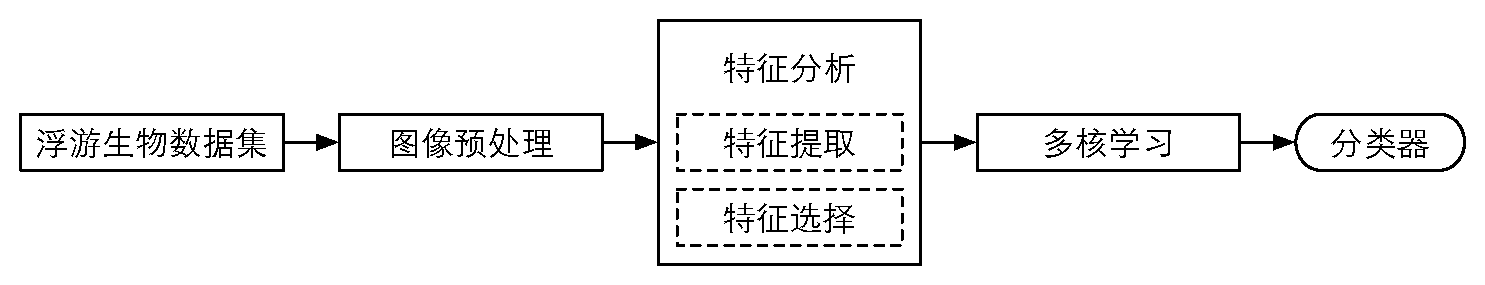
\includegraphics[width=1\linewidth]{frame}
\end{figure}
% \begin{enumerate}
% \item 图像预处理
% \item 特征分析
% \item 多核学习
% \end{enumerate}
% \end{column}
% \end{columns}\vspace{1ex}
\end{frame}

%\subsection{图像预处理}

\begin{frame}
\frametitle{\ding{172}图像预处理}
\begin{enumerate}
\item {\color{blue}图像分割}\footnote{Sosik H M, Olson R J. Automated taxonomic classification of phytoplankton sampled with imaging-in-flow cytometry. Limnol. Oceanogr. Methods, 2007, 5(204):e216.} 对未分割的图像进行分割

\begin{figure}
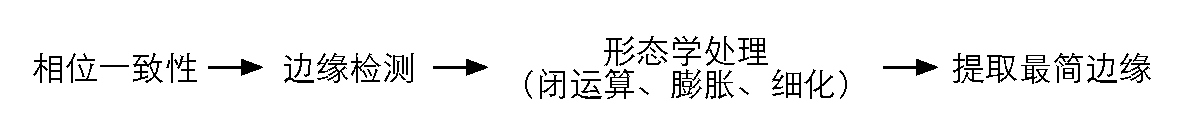
\includegraphics[width=0.9\linewidth]{imgpro}
\end{figure}

%相位一致性 $\to$ 边缘检测 $\to$ 形态学处理(闭运算、膨胀、细化) $\to$ 提取最简边缘

\item {\color{blue}去除悬浮颗粒等杂质} 开运算,去除小连通区域
\end{enumerate}
\end{frame}

%\subsection{特征提取}

\begin{frame}
\frametitle{\ding{173}浮游生物特征分析}
\shadow{特征提取}

{\color{blue}{\ding{172}~几何灰度特征}}

周长、面积、体态比、灰度平均值、灰度标准差$\cdots$共43个。\\
~

{\color{blue}{\ding{173}~粒子测度}}

用来计算二值图像中目标区域的大小分布情况。
% \begin{displaymath}

% \end{displaymath}
\begin{displaymath}
F_{G}(\lambda) = 1-\frac{v(\psi_{\lambda}(G))}{v(G)} ~~~~ \psi_{\lambda}(G) = G\circ\lambda T
\end{displaymath}
\end{frame}

\begin{frame}
\frametitle{\ding{173}浮游生物特征分析}
\begin{columns}
\begin{column}{0.5\linewidth}
{\color{blue}{\ding{174}~纹理特征}}
\begin{itemize}
\item 变差函数
\item Gabor滤波器
\item 局部二值模式
\item 二元梯度轮廓
\end{itemize}
\end{column}
\begin{column}{0.5\linewidth}
{\color{blue}{\ding{175}~局部特征}}
\begin{itemize}
\item 内距离形状上下文
\item 方向梯度直方图
\item 尺度不变特征变换
\end{itemize}
\end{column}
\end{columns}\vspace{1ex}

~\\
\pause

\shadow{特征选择}

从特征集合中选取有用的特征子集,去除冗余特征,降低特征维数。
\end{frame}

%\subsection{特征选择}





% \begin{enumerate}
% \item 生成子集:选取特征子集
% \item 评价函数:评价特征子集的好坏
% \item 停止准则:评价结果达到一定标准后停止搜索
% \item 验证过程:验证选出的特征子集的有效性
% \end{enumerate}


%\subsection{多核学习}

\begin{frame}
\frametitle{\ding{174}多核学习}
机器学习中常用的{\color{blue}支持向量机}是{\color{red}单核}学习算法。\\
~

{\color{blue}多核学习}用多个核函数的组合代替单个核函数。
\begin{figure}
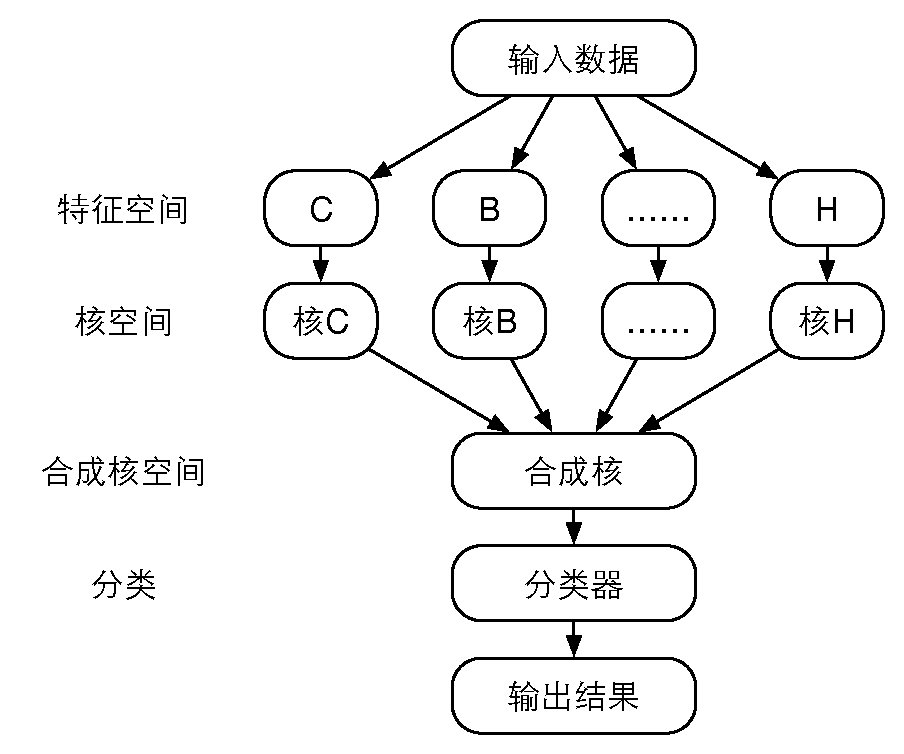
\includegraphics[width=0.5\linewidth]{multikernel}
\end{figure}
\end{frame}

\subsection{评价方法}

\begin{frame}
\frametitle{混淆矩阵}
一种特定的矩阵用来呈现算法性能的可视化工具。

%\centering {\color{blue}混淆矩阵}
\begin{table}[htbp]
  \centering
  %\caption{混淆矩阵}
  \begin{tabular}[c]{cccc}
    %\hline
    \toprule
    \multicolumn{2}{c}{\multirow{2}*{~}} & \multicolumn{2}{c}{预测结果}\\
    %\cline{3-4}
    \multicolumn{2}{c}{~} & 正样本 & 负样本\\
    %\hline
    \midrule
    \multirow{2}*{实际结果} & 正样本 & a & b\\
    %\cline{2-4}
     & 负样本 & c & d\\
    \bottomrule
    %\hline
  \end{tabular}
\end{table}

\begin{itemize}
\item {\color{blue}真阳性率}(True positive rate,也称召回率Recall):
  \begin{displaymath}
    TPR = \frac{a}{a+b}
  \end{displaymath}
\item {\color{blue}阳性预测值}(Positive predictive value,也称为命中率Precision):
  \begin{displaymath}
    Precision = \frac{a}{a+c}
  \end{displaymath}
\end{itemize}
\end{frame}

\begin{frame}
\frametitle{F-Measure}
{\color{blue}F-Measure}是一种综合评价指标。\\
~

当Recall和Precision出现矛盾时,就可以采用该方法进行评价。
\begin{displaymath}
F=\frac{(\alpha^{2}+1)P*R}{\alpha^{2}(P+R)}
\end{displaymath}
当$\alpha=1$就得到F1-Measure:
\begin{displaymath}
F1=\frac{2*PR}{P+R}
\end{displaymath}
\end{frame}

\section{对比实验及结果分析}

%\subsection{对比实验}
\begin{frame}
\frametitle{对比实验}
\begin{enumerate}
\item 基准实验
\item 特征对比实验
\item 基于多核学习的浮游生物图像分类实验
\end{enumerate}
\end{frame}

\begin{frame}
\frametitle{\ding{172}基准实验}
根据Sosik等人在2007年提出的浮游植物自动分类方法\footnote{Sosik H M, Olson R J. Automated taxonomic classification of phytoplankton sampled with imaging-in-flow cytometry. Limnol. Oceanogr. Methods, 2007, 5(204):e216.}和ZooScan系统\footnote{Gorsky G, Ohman M D, Picheral M, et al. Digital zooplankton image analysis using the zooscan integrated system. Journal of Plankton Research, 2010, 32(3):285–303.}设计浮游生物分类基准系统。
\begin{figure}
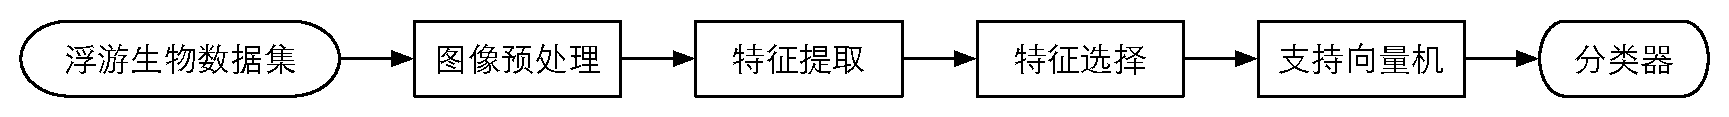
\includegraphics[width=1\linewidth]{jizhun}
\end{figure}
\shadow{基准实验结果}
\begin{table}[htbp]
  % \small
  \scriptsize
  \centering
  %\caption{基准系统的分类结果}
  \begin{tabular}[c]{cccc}
    \toprule
    %\hline
    ~ & WHOI数据集 & ZooScan数据集 & Kaggle数据集\\
    \midrule
    %\hline
    %Recall & 88.27\% & 80.6\% & 75.36\%\\
    %\hline
    %1-Precision & 11.63\% & 16.3\% & 21.49\%\\
    %Precision & 88.37\% & 83.7\% & 78.51\%\\
    F-Measure & 0.8832~{\color{blue}(0.8792)} & 0.8212~{\color{blue}(0.7947)} & 0.7690\\
    \bottomrule
    %\hline
  \end{tabular}
\end{table}
\end{frame}

\begin{frame}
\frametitle{\ding{173}特征对比实验}
\begin{columns}
\begin{column}{0.4\linewidth}
%在基准实验的基础上设计特征对比实验,对设计系统的特征提取部分的性能进行评价。
\begin{figure}
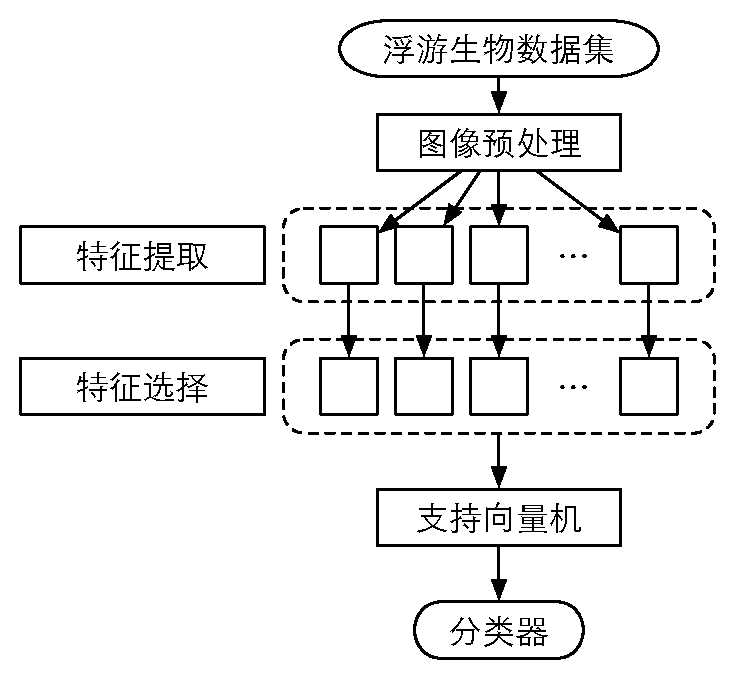
\includegraphics[width=0.85\linewidth]{shiyan2}
\end{figure}
\end{column}

\begin{column}{0.6\linewidth}
\centering \small{特征对比实验结果}
\begin{table}[htbp]
\tiny
  \centering
  \begin{tabular}[c]{ccccc}
    \toprule
    %\hline
    \multirow{2}*{数据集} & \multirow{2}*{C} & 高斯核函数 & 多项式核函数 & 线性核函数\\
    %\cline{3-8}
     & & F-Measure & F-Measure & F-Measure\\
    \midrule
    %\hline
    \multirow{3}*{WHOI数据集} & 1 & 0.8428 & 0.8901 & 0.8652\\
    %\cline{2-8}
     & 10 & 0.8897 & 0.8949 & 0.8817\\
    %\cline{2-8}
     & 100 & {\color{red}0.8963} & 0.8848 & 0.8637\\
    \midrule
    %\hline
    \multirow{3}*{ZooScan数据集} & 1 & 0.8174 & 0.8322 & 0.8087\\
    %\cline{2-8}
     & 10 & {\color{red}0.8609} & 0.8446 & 0.8475\\
    %\cline{2-8}
     & 100 & 0.8562 & 0.8351 & 0.8202\\
    \midrule
    %\hline
    \multirow{3}*{Kaggle数据集} & 1 & 0.7910 & 0.7891 & 0.7307\\
    %\cline{2-8}
     & 10 & {\color{red}0.8304} & 0.8131 & 0.7890\\
    %\cline{2-8}
     & 100 & 0.8260 & 0.7964 & 0.7802\\
    \bottomrule
    %\hline
  \end{tabular}
\end{table}
\end{column}
\end{columns}\vspace{1ex}
\end{frame}

\begin{frame}
\begin{columns}
\begin{column}{0.5\linewidth}
\begin{figure}
\includegraphics[width=0.8\linewidth]{comp12}
\end{figure}
\end{column}

\begin{column}{0.5\linewidth}
\centering{对比实验\ding{172}\ding{173}}
\begin{table}
\scriptsize
  \centering
  % \caption{对比实验\ding{172}\ding{173}}
  \begin{tabular}[c]{cc}
    \toprule
    %\hline
    数据集 & F-Measure提高量\\
    \midrule
    %\hline
    WHOI数据集 & 0.0131\\
    %\hline
    ZooScan数据集 & 0.0397\\
    %\hline
    Kaggle数据集 & 0.0641\\
    \bottomrule
    %\hline
  \end{tabular}
\end{table}
\end{column}
\end{columns}\vspace{1ex}
\end{frame}

% \begin{frame}
% \frametitle{\ding{174}基于多核学习的浮游生物图像分类实验}
% 采用一种核函数的基于多核学习的浮游生物分类系统
% \begin{columns}
% \begin{column}{0.4\linewidth}
% \begin{figure}
% 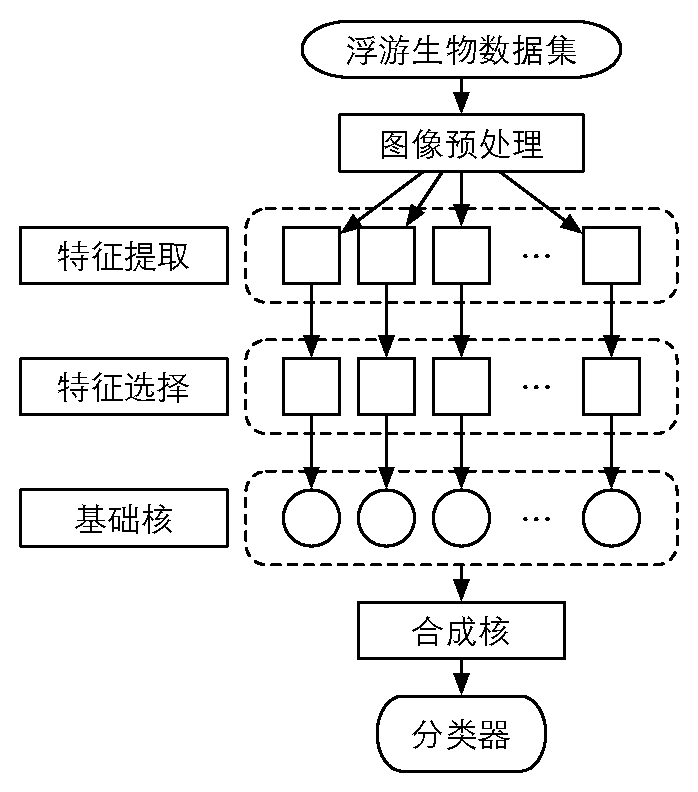
\includegraphics[width=0.8\linewidth]{shiyan31}
% \end{figure}
% \end{column}

% \begin{column}{0.6\linewidth}
% \begin{table}[htbp]
% \tiny
%   \centering
%   \caption{实验结果}
%   \begin{tabular}[c]{ccccc}
%     \toprule
%     %\hline
%     \multirow{2}*{数据集} & \multirow{2}*{C} & 高斯核函数 & 多项式核函数 & 线性核函数\\
%     %\cline{3-8}
%      & & F-Measure & F-Measure & F-Measure\\
%     \midrule
%     %\hline
%     \multirow{3}*{WHOI数据集} & 1 & 88.56\% & 89.68\% & 88.68\%\\
%     %\cline{2-8}
%      & 10 & 88.85\% & {\color{red}89.75\%} & 89.23\%\\
%     %\cline{2-8}
%      & 100 & 88.69\% & 89.47\% & 88.5\%\\
%     \midrule
%     %\hline
%     \multirow{3}*{ZooScan数据集} & 1 & 85.72\% & 85.53\% & 83.1\%\\
%     %\cline{2-8}
%      & 10 & 88.09\% & 87.48\% & 84.35\%\\
%     %\cline{2-8}
%      & 100 & {\color{red}88.31\%} & 87.57\% & 83.94\%\\
%     \midrule
%     %\hline
%     \multirow{3}*{Kaggle数据集} & 1 & 80.47\% & 81.79\% & 79.4\%\\
%     %\cline{2-8}
%      & 10 & 83.26\% & {\color{red}83.48\%} & 81.83\%\\
%     %\cline{2-8}
%      & 100 & 83.06\% & 83.13\% & 80.29\%\\
%     \bottomrule
%     %\hline
%   \end{tabular}
% \end{table}

% \end{column}
% \end{columns}\vspace{1ex}
% \end{frame}

% \begin{frame}
% \begin{columns}
% \begin{column}{0.5\linewidth}
% \begin{figure}
% \includegraphics[width=0.8\linewidth]{comp23}
% \end{figure}
% \end{column}

% \begin{column}{0.5\linewidth}
% \begin{table}
% \scriptsize
%   \centering
%   \caption{对比实验\ding{173}\ding{174}}
%   \begin{tabular}[c]{cc}
%     \toprule
%     %\hline
%     数据集 & F-Measure\\
%     \midrule
%     %\hline
%     WHOI数据集 & 0.12\%\\
%     %\hline
%     ZooScan数据集 & 1.22\%\\
%     %\hline
%     Kaggle数据集 & 0.44\%\\
%     \bottomrule
%     %\hline
%   \end{tabular}
% \end{table}
% \end{column}
% \end{columns}\vspace{1ex}
% \end{frame}

\begin{frame}
\frametitle{\ding{174}基于多核学习的浮游生物图像分类实验}
%结合三种核函数的基于多核学习的浮游生物分类系统
\begin{columns}
\begin{column}{0.6\linewidth}
\begin{figure}
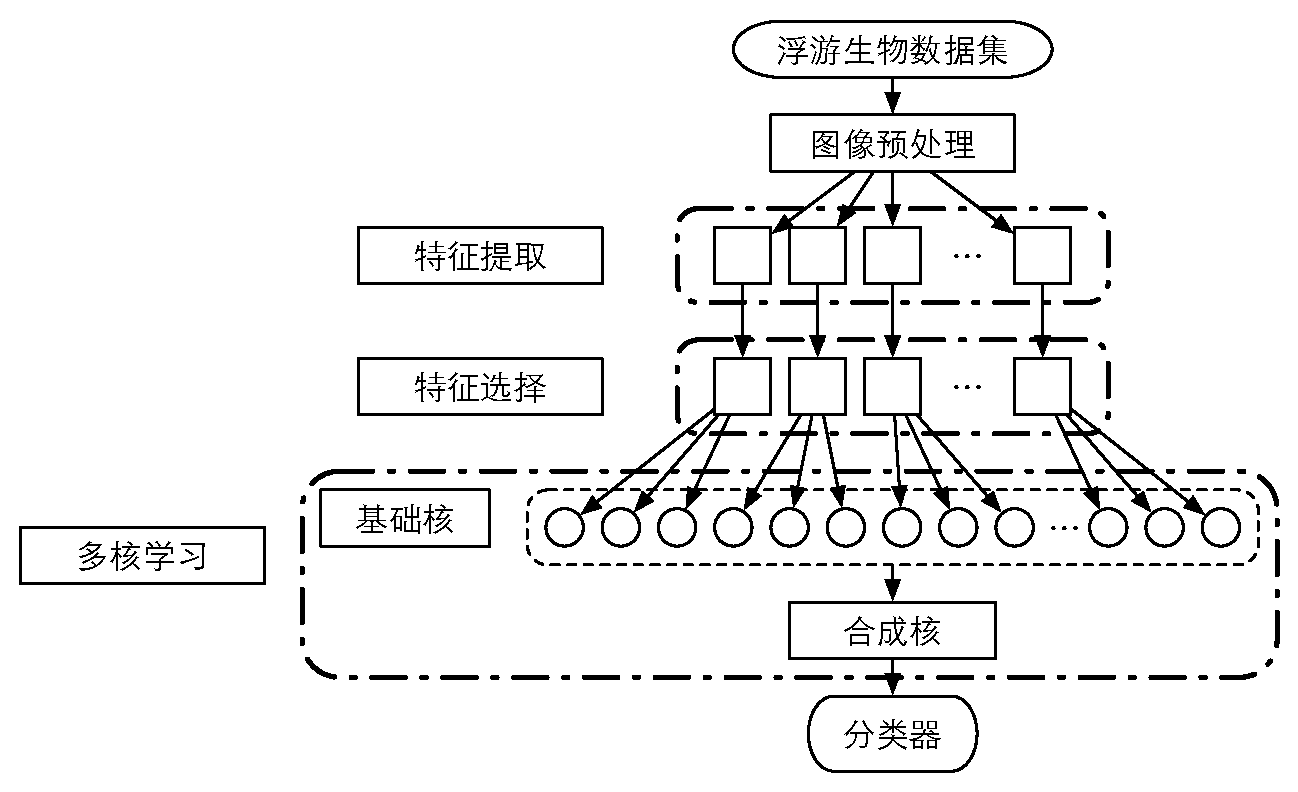
\includegraphics[width=1\linewidth]{shiyan32}
\end{figure}
\end{column}

\begin{column}{0.5\linewidth}
\centering{\small{实验结果}}
\begin{table}[htbp]
\tiny
  \centering
  %\caption{实验结果}
  \begin{tabular}[c]{ccc}
    \toprule
    %\hline
    数据集 & C & F-Measure\\
    \midrule
    %\hline
    \multirow{3}*{WHOI数据集} & 1 & 0.8973\\
    %\cline{2-4}
     & 10 & 0.8992\\
    %\cline{2-4}
     & 100 & {\color{red}0.9004}\\
    \midrule
    %\hline
    \multirow{3}*{ZooScan数据集} & 1 & 0.8699\\
    %\cline{2-4}
     & 10 & {\color{red}0.8937}\\
    %\cline{2-4}
     & 100 & 0.8924\\
    \midrule
    %\hline
    \multirow{3}*{Kaggle数据集} & 1 & 0.8205\\
    %\cline{2-4}
     & 10 & {\color{red}0.8458}\\
    %\cline{2-4}
     & 100 & 0.8428\\
    \bottomrule
    %\hline
  \end{tabular}
\end{table}
\end{column}
\end{columns}\vspace{1ex}
\end{frame}

\begin{frame}
\begin{columns}
\begin{column}{0.5\linewidth}
\begin{figure}
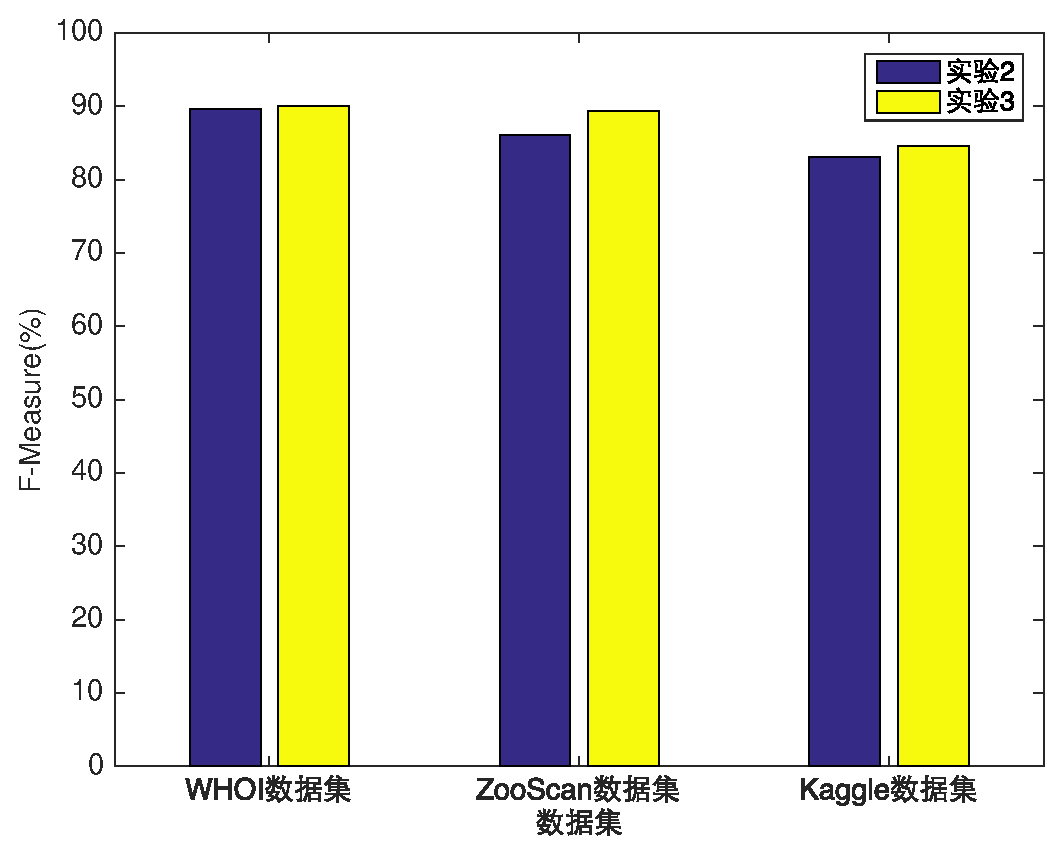
\includegraphics[width=0.7\linewidth]{comp232}
\end{figure}
\end{column}

\begin{column}{0.5\linewidth}
\centering{对比实验\ding{173}\ding{174}}
\begin{table}
\scriptsize
  \centering
  %\caption{对比实验\ding{173}\ding{174}}
  \begin{tabular}[c]{cc}
    \toprule
    %\hline
    数据集 & F-Measure提高量\\
    \midrule
    %\hline
    WHOI数据集 & 0.0041\\
    %\hline
    ZooScan数据集 & 0.0328\\
    %\hline
    Kaggle数据集 & 0.0154\\
    \bottomrule
    %\hline
  \end{tabular}
\end{table}
\end{column}
\end{columns}\vspace{1ex}
\pause
\begin{columns}
\begin{column}{0.5\linewidth}
\begin{figure}
\includegraphics[width=0.7\linewidth]{comp13}
\end{figure}
\end{column}

\begin{column}{0.5\linewidth}
\centering{对比实验\ding{172}\ding{174}}
\begin{table}
\scriptsize
  \centering
  %\caption{对比实验\ding{172}\ding{174}}
  \begin{tabular}[c]{cc}
    \toprule
    %\hline
    数据集 & F-Measure提高量\\
    \midrule
    %\hline
    WHOI数据集 & 0.0172\\
    %\hline
    ZooScan数据集 & 0.0725\\
    %\hline
    Kaggle数据集 & 0.0768\\
    \bottomrule
    %\hline
  \end{tabular}
\end{table}
\end{column}
\end{columns}\vspace{1ex}
\end{frame}

% \begin{frame}
% \begin{columns}
% \begin{column}{0.5\linewidth}
% \begin{figure}
% 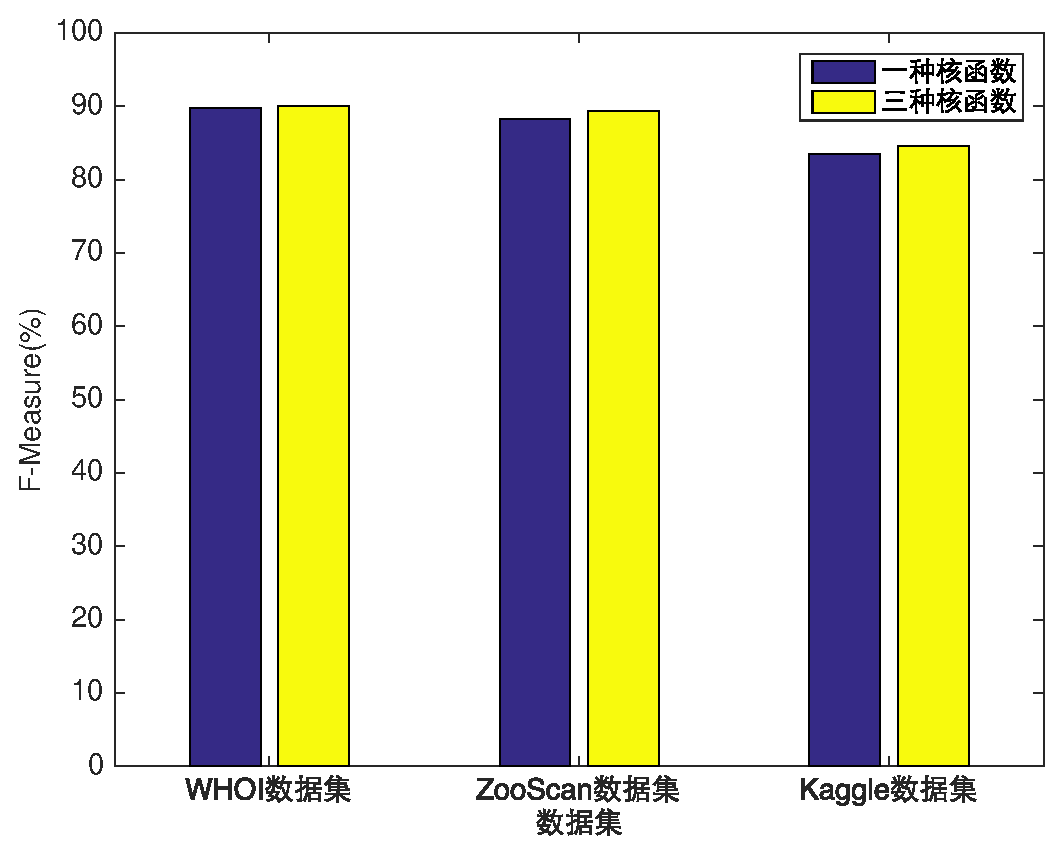
\includegraphics[width=0.7\linewidth]{comp3}
% \end{figure}
% \end{column}

% \begin{column}{0.5\linewidth}
% \begin{table}
% \scriptsize
%   \centering
%   \caption{对比实验\ding{174}}
%   \begin{tabular}[c]{cc}
%     \toprule
%     %\hline
%     数据集 & F-Measure\\
%     \midrule
%     %\hline
%     WHOI数据集 & 0.29\%\\
%     %\hline
%     ZooScan数据集 & 1.06\%\\
%     %\hline
%     Kaggle数据集 & 1.1\%\\
%     \bottomrule
%     %\hline
%   \end{tabular}
% \end{table}
% \end{column}
% \end{columns}\vspace{1ex}
% \pause
% \begin{columns}
% \begin{column}{0.5\linewidth}
% \begin{figure}
% \includegraphics[width=0.7\linewidth]{comp13}
% \end{figure}
% \end{column}

% \begin{column}{0.5\linewidth}
% \begin{table}
% \scriptsize
%   \centering
%   \caption{对比实验\ding{172}\ding{174}}
%   \begin{tabular}[c]{cc}
%     \toprule
%     %\hline
%     数据集 & F-Measure\\
%     \midrule
%     %\hline
%     WHOI数据集 & 1.72\%\\
%     %\hline
%     ZooScan数据集 & 7.25\%\\
%     %\hline
%     Kaggle数据集 & 7.68\%\\
%     \bottomrule
%     %\hline
%   \end{tabular}
% \end{table}
% \end{column}
% \end{columns}\vspace{1ex}
% \end{frame}

\section{总结与展望}

\begin{frame}
\frametitle{总结与展望}
\begin{tcolorbox}[colback=red!5,colframe=blue!75!black]
\shadow{总结}
\begin{itemize}
\item 分析浮游生物形态特征,从多角度对浮游生物进行描述。
\item 提出基于多核学习的浮游生物自动分类系统。
\item 收集构建不同的浮游生物数据集,设计对比实验评价分类性能。
\end{itemize}
\end{tcolorbox}
\begin{tcolorbox}[colback=red!5,colframe=blue!75!black]
\shadow{展望}
\begin{itemize}
\item 提高分类系统的计算效率。
\item 针对数据集不均衡问题进行进一步研究。
\end{itemize}
\end{tcolorbox}
\end{frame}

\begin{frame}
\vspace{2cm}

\centering{\shado{\textit{谢谢!}}}
%\centering{\color{blue} \kaishu \Huge{ \emph{\textbf{  谢谢!}}}}\\
\vspace{1.5cm}

\begin{flushright}
\emph{\href{mailto:wangruchen514@163.com}{\textrm {Ruchen~Wang}}}\\
\href{http://www.ouc.edu.cn}{\textrm {Ocean University of China}}\\
\emph{\textrm {2017.05}}
\end{flushright}  
\end{frame}

\end{document}
